\section{Convertir entre RGB e YUV}

Los primeros filtros se tratan de conversores entre los espacios de colores RGB e YUV. Los mismos toman los valores de cada pixel y aplican transformaciones matriciales, tomando cada pixel individual como una matriz de sus componentes.

Esta transformación normalmente implica decimales, pero la misma está simplificada para funcionar con enteros entre 0 y 255 (que son los valores posibles de cada componente de un pixel).

Para la conversión RGB a YUV se aplican la siguiente transformación:

\begin{center}

	$
	\begin{bmatrix*}[l]
	Y = sature(((66 * R + 129 * G + 25 * B + 128) >> 8) + 16) \\
	U = sature(((-38 * R - 74 * G + 112 * B + 128) >> 8) + 128) \\
	V = sature(((112 * R - 94 * G - 18 * B + 128) >> 8) + 128)
	\end{bmatrix*}
	$

\end{center}

donde $sature$ representa una saturación sin signo, es decir, los valores fuera del rango [0,255] son acotados a los extremos del mismo.

Para la transformación inversa se utiliza la siguiente transformación:

\begin{center}

	$
	\begin{bmatrix*}[l]
	R = sature((298 * (Y - 16) + 409 * (V - 128) + 128) >> 8) \\
	G = sature((298 * (Y - 16) - 100 * (U - 128) - 208 * (V - 128) + 128) >> 8) \\
	B = sature((298 * (Y - 16) + 516 * (U - 128) + 128) >> 8)
	\end{bmatrix*}
	$

\end{center}

Cabe destacar que si bien los valores son correctos, los visores de imágenes siguen renderizando los colores como si correspondiesen a RGB, por lo que se genera el efecto visual que se muestra a continuación:


\begin{figure}[H]
	\centering
	$\vcenter{\hbox{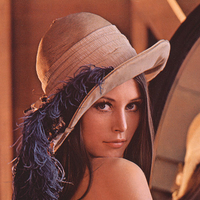
\includegraphics[scale=1]{img/convert_RGB.jpg}}}$
	$\vcenter{\hbox{\LARGE$\xrightleftharpoons[\text{YUVtoRGB}]{\text{RGBtoYUV}}$}}$
	$\vcenter{\hbox{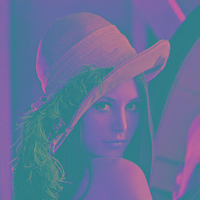
\includegraphics[scale=1]{img/convert_YUV.jpg}}}$
\end{figure}


\subsection{Implementación}

La solución implica recorrer la imagen completa aplicando la transformación a cada pixel de manera individual.

La implementación en C es relativamente trivial: se aplica la transformación correspondiente a cada componente de manera individual. En el caso de la transformación YUV a RGB existen algunos valores que podemos reutilizar, pero los demás cálculos se realizan como se indica en el problema.

Para la implementación en ASM definimos un par de constantes. La idea es que cada una represente una fila de la matriz de transformación. De esta manera, podemos calcular los 3 componentes fuente de cada componente destino en simultaneo.

Para los siguientes ejemplos se utiliza el filtro RGB2YUV, pero la implementación del filtro inverso es muy similar.

Primero, se definen 3 máscaras. Cada una se utilizará para crear una de las componentes finales:

\begin{center}
	\xmm{9} \xmmDoubleWordSmall{66}{129}{25}{0}

	\xmm{10} \xmmDoubleWordSmall{-38}{-74}{112}{0}

	\xmm{11} \xmmDoubleWordSmall{112}{-94}{-18}{0}
\end{center}

Ya que contamos con registros de 128 bits y cada pixel mide 32 bits de ancho (RGBA), podemos cargar 4 pixeles de la memoria por iteración. Esto permite reducir el impacto de los accesos a memoria y los saltos condicionales.

No obstante, los mismos son desempaquetados para ocupar los registros XMM de manera individual, con cada una de sus componentes en tamaño doubleword (32 bits). Esto es porque los valores que multiplicamos y sumamos pueden exceder el límite de una word, y perderíamos precisión o retornaríamos valores inválidos. Esto también se refleja en la implementación C, donde consideramos utilizar \texttt{unsigned short}, de 16 bits, pero esto generaba demasiados errores y nos vimos forzados a usar \texttt{unsigned int}, de 32 bits.

Por lo tanto, la lógica de procesamiento de cada pixel se ve repetida 4 veces, una por pixel por iteración. Sin embargo, tenemos la garantía que la imagen tendrá como ancho un múltiplo de 4, por lo que esto no presenta un problema.

\begin{center}

	\xmm{0} \xmmDoubleWordSmall{0}{0}{0}{0}

	\xmm{4} \xmmDoubleWordSmall{P1}{P2}{P3}{P4}

	\xmm{2} $\leftarrow$ \xmm{4}

	\texttt{PUNPCKHBW} \xmm{2}, \xmm{0} \hfill

	\xmm{2} \xmmWord{$P1_R$}{$P1_G$}{$P1_B$}{0}{$P2_R$}{$P2_G$}{$P2_B$}{0}

	\xmm{1} $\leftarrow$ \xmm{2}

	\texttt{PUNPCKHWD} \xmm{1}, \xmm{0} \hfill

	\texttt{PUNPCKLWD} \xmm{2}, \xmm{0} \hfill

	\xmm{1} \xmmDoubleWordSmall{$P1_R$}{$P1_G$}{$P1_B$}{0}

	\xmm{2} \xmmDoubleWordSmall{$P2_R$}{$P2_G$}{$P2_B$}{0}

	$\vdots$

	(se omiten instrucciones por su similitud)

	\xmm{3} \xmmDoubleWordSmall{$P3_R$}{$P3_G$}{$P3_B$}{0}

	\xmm{4} \xmmDoubleWordSmall{$P4_R$}{$P4_G$}{$P4_B$}{0}

\end{center}

Cada pixel es copiado 3 veces (en su registro original y a los registros XMM14 y XMM15), una por componente destino (en este caso, Y, U y V). Luego, se multiplican estas copias del pixel por la máscara correspondiente:

\begin{center}

	\texttt{PMULLD} \xmm{14}, \xmm{9} \hfill

	\xmm{14} \xmmDoubleWordSmall{$Y'_R$}{$Y'_G$}{$Y'_B$}{0}

	\texttt{PMULLD} \xmm{15}, \xmm{10} \hfill

	\xmm{15} \xmmDoubleWordSmall{$U'_R$}{$U'_G$}{$U'_B$}{0}

	\texttt{PMULLD} \xmm{1}, \xmm{11} \hfill

	\xmm{1} \xmmDoubleWordSmall{$V'_R$}{$V'_G$}{$V'_B$}{0}
	
\end{center}

Por último, estos valores intermedios se suman horizontalmente para crear las componentes finales:

\begin{center}

	\texttt{PHADDD} \xmm{15}, \xmm{14} \hfill

	\xmm{15} \xmmDoubleWordSmall{$Y'_{R+G}$}{$Y'_B$}{$U'_{R+G}$}{$U'_B$}

	\texttt{PHADDD} \xmm{1}, \xmm{1} \hfill

	\xmm{1} \xmmDoubleWordSmall{$V'_{R+G}$}{$V'_B$}{$V'_{R+G}$}{$V'_B$}

	\texttt{PHADDD} \xmm{1}, \xmm{15} \hfill

	\xmm{1} \xmmDoubleWordSmall{$Y'$}{$U'$}{$V'$}{$V'$}

\end{center}

Como se puede ver, al sumar se genera un valor duplicado al final. El mismo se genera porque las imagenes tienen 3 componentes y \texttt{PHADDD} toma siempre 2 parámetros. Esto no afecta la correción del filtro, ya que no estamos trabajando con el componente alfa y el mismo puede ser descartado.

Por último, estos componentes se denotan con $'$ porqe los mismos no son los valores finales: debemos aplicar 2 sumas y un shift a todos los componentes para finalizar la conversión. Para las sumas utilizamos nuevamente constantes precargadas en un registro XMM.

Al finalizar la conversión, los pixeles son reempaquetados para ser guardados en una sola operación. El empaquetado es sin signo, de manera que cualquier valor por encima del máximo es acotado al máximo de dicha componente (\texttt{0xFF}):

\begin{center}
	\xmm{1} \xmmDoubleWordSmall{$P1_Y$}{$P1_U$}{$P1_V$}{0}

	\xmm{2} \xmmDoubleWordSmall{$P2_Y$}{$P2_U$}{$P2_V$}{0}

	\xmm{3} \xmmDoubleWordSmall{$P3_Y$}{$P3_U$}{$P3_V$}{0}

	\xmm{4} \xmmDoubleWordSmall{$P4_Y$}{$P4_U$}{$P4_V$}{0}

	\texttt{PACKUSDW} \xmm{2}, \xmm{1} \hfill

	\xmm{2} \xmmWord{$P1_Y$}{$P1_U$}{$P1_V$}{0}{$P2_Y$}{$P2_U$}{$P2_V$}{0}

	\texttt{PACKUSDW} \xmm{4}, \xmm{3} \hfill

	\xmm{4} \xmmWord{$P3_Y$}{$P3_U$}{$P3_V$}{0}{$P4_Y$}{$P4_U$}{$P4_V$}{0}

	\texttt{PACKUSWB} \xmm{4}, \xmm{2} \hfill

	\xmm{4} \xmmDoubleWordSmall{P1}{P2}{P3}{P4}
\end{center}

(notese que en este contexto $Pi$ no representa el mismo pixel de entrada sino su correspondiente post-conversión)

Un detalle importante que aplica a este filtro es la independencia entre todos los pixeles, y la independencia de los mismos con respecto a su posición. Este detalle nos permite recorrer la imagen no como una matriz de pixeles sino como una lista continua de tamaño $w \times h$.

\subsection{Análisis preliminar}

Para realizar un análisis preliminar del rendimiento de los algoritmos, debimos medir los tiempos de ejecución de los mismos. Por claridad, unificamos el criterio utilizados para las mediciones a lo largo de todo el trabajo práctico. Los detalles de dicho critero se encuentran en el apéndice correspondiente.

Como ambos filtros son muy similares, los podemos comparar lado a lado:

\begin{center}
	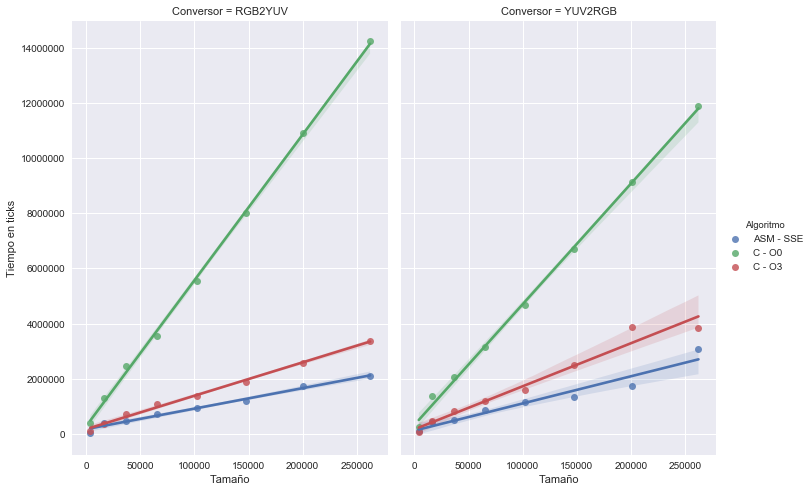
\includegraphics[scale=0.5]{img/conversores_CvsASMvsO3.png}
\end{center}

Lo primero que se puede apreciar en este gráfico es que, más allá de la implementación utilizada, el tiempo de ejecución del filtro aumenta de forma lineal con el tamaño de la imagen, en este caso medido en pixeles. Cabe destacar que en nuestras mediciones, los casos de imágenes pequeñas dieron resultados dispares, pero para el resto de los tamaños esta tendencia se mantiene.

Para continuar, se puede notar una diferencia enorme en la performance del algoritmo escrito en C contra el escrito en ASM. Al compilar con optimizaciones, la brecha de performance baja drásticamente. Sospechamos que esto se debe a un uso más exhaustivo de los registros en lugar de acceder constantemente a memoria. Sin embargo, se puede ver que el algoritmo escrito con instrucciones SIMD sigue siendo más óptimo. Decidimos analizar esto más de cerca:

\begin{center}
	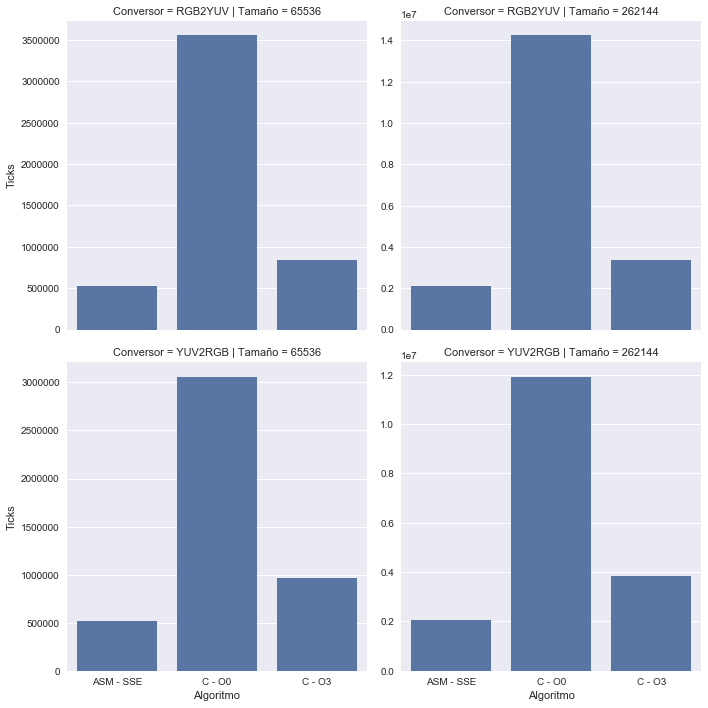
\includegraphics[scale=0.5]{img/conversores_CvsASMvsO3_bars.png}
\end{center}

Este gráfico nos muestra de forma clara que el filtro escrito en ASM se ejecuta en entre 50\% y 70\% del tiempo al compararlo con el filtro en C compilado con el flag \texttt{-O3}. Si bien ambos filtros se ejecutan varias veces más rápido que la versión sin optimizaciones de compilador (\texttt{-O0}), la diferencia porcentual entre ellos es visible y relevante.

Por otro lado, se puede ver que en O0 el conversor YUV a RGB performa mejor que su contraparte RGB a YUV (con una diferencia de más de 10\%). Esto posiblemente se deba a ciertas operaciones que como mencionamos se repiten, y por ende podemos pre-calcular y reutilizar valores intermedios.

\subsection{Experimentación}

A modo de experimentación, decidimos probar 2 hipótesis distintas:

\subsubsection*{Hipótesis 1: cargar 4 pixeles a la vez mejora la performance}

Como se mencionó en la sección de implementación, en nuestra implementación cargamos 4 pixeles de la memoria a los registros XMM, para luego desempaquetarlos y procesarlos de manera individual. Nosotros hicimos esto bajo la hipótesis que reducir los saltos y los accesos a memoria mejoraría el rendimiento de los filtros.

Decidimos comprobar esta teoría implementando los mismos filtros pero cargando y procesando 1 único pixel por iteración:

\begin{center}
	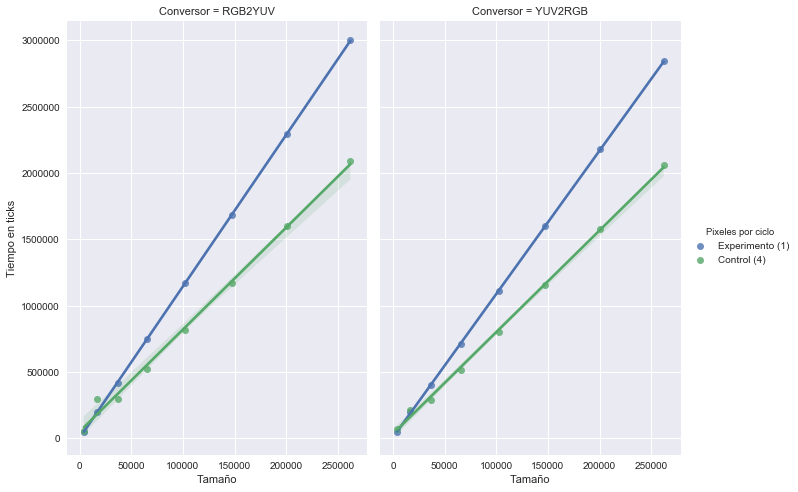
\includegraphics[scale=0.5]{img/conversores_1pixel.png}
\end{center}

Efectivamente, las implementaciones más veloces son aquellas que aprovechan la instrucción \texttt{movdqu} para cargar 4 pixeles con un solo acceso a memoria, y que consecuentemente procesan 4 pixeles sin hacer saltos.

Por otro lado, al acceder de manera lineal a la memoria, el caché debería mitigar una gran candidad de esos accesos, así que es posible que el impacto mayor no provenga necesariamente de los accesos a memoria, sino de los saltos condicionales.

\subsubsection*{Hipótesis 2: los filtros corren en tiempos uniformes para toda imagen de mismo tamaño}

De cara a la experimentación, esperábamos que los algoritmos fuesen agnósticos a la composición de la imagen de entrada, es decir, de los pixeles particulares que la componen. Si bien sabemos que el tamaño de la imagen si afecta de forma lineal el tiempo de ejecución, supusimos que los colores que componen las imágenes no modificarían dicho tiempo.

Para comprobar esta teoría, probamos correr el conversor sobre utilizando un bitmap blanco. Corrimos los mismos conversores, en ambas implementaciones:

\begin{center}
	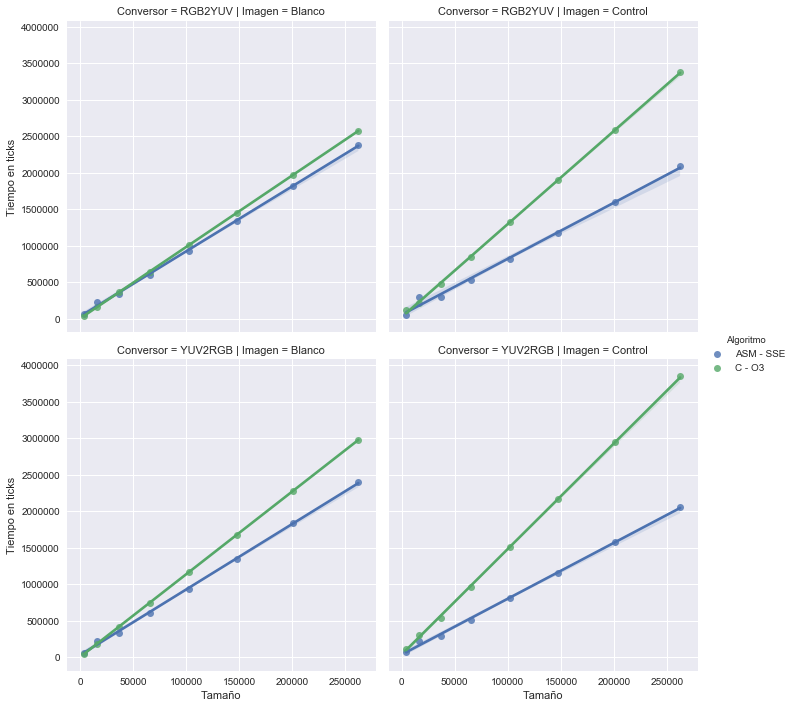
\includegraphics[scale=0.5]{img/conversores_blanco.png}
\end{center}

Para nuestra sorpresa, podemos ver que la saturación de las componentes tiene un efecto visible en el tiempo de ejecución de los filtros. No solo eso, el bitmap afecta de manera positiva a la implementación en C, mientras que impacta de forma negativa a su contraparte SSE.

Este dato nos tomó por sorpresa, y aunque intentamos analizar el por qué de este impacto, no pudimos dilucidar la causa. De un modo u otro, esto muestra que la imagen de entrada pueden afectar notoriamente la performance de los filtros, negando nuestra hipótesis inicial.